\chapter{LTL Tool over Petri nets}\label{chltl}
In this chapter, we elaborate on the first contribution of the thesis - bounded model checking of unbounded Petri nets with concurrent semantics.
First, we discuss bounded model checking for various properties on Petri nets. Second, we provide the SMT encoding for unbounded Petri nets and their concurrent unfolding. Third, we describe the model checking tool for verifying temporal properties (expressed in LTL with linear integer arithmetic) for unbounded Petri nets and discuss the experimental results.

% \todo{Talk about concurrent semantics in the context of Petri nets, historically.}
\section{Bounded Model Checking for unbounded PNs}


The intuition behind BMC and its extension, $2D$-BMC is to represent a counterexample-trace of bounded length symbolically and check the resulting formula with a SAT/SMT solver. If the formula is satisfiable and thus the path feasible, a satisfying assignment returned by the solver can be translated into a concrete counterexample trace that shows that the property is violated. Otherwise, the bound is increased and the process repeated. Complete extensions to this approach allow to stop this process at one point, with the conclusion that the property cannot be violated, hopefully before the available resources are exhausted. The details of $2D$-BMC are discussed in detail in Sec.~\ref{secbmcalgo}. In this section, we focus on performing $2D$-BMC on unbounded Petri nets, taking advantage of true concurrency in the nets and representing the properties of the nets in a temporal logic {\LC}. Linear Temporal Logic ($LTL$)~\cite{P77,VardiW86} is a natural choice to describe temporal properties of unbounded systems. While $LTL$ is useful to us, we cannot express any counting properties, hence, we propose using the counting logic language {\LC} an extension of $LTL$ with a few
differences (cf. Sec.~\ref{sec:cltl}). In the case of $LTL$, atomic formulas are propositional
constants which have no further structure. The syntax of the logic is explained with respect to client-server systems, but is also applicable in other infinite state systems such as Fig.~\ref{fig:APS}. In {\LC}, there are three types of atomic formulas: (1) describing basic server properties, $P_s$ which are propositional constants (2) {\bf counting} sentences of the kinds
$(\mbox{\#} x >\mathfrak{c})\alpha$ and $(\mbox{\#} x \le \mathfrak{c})\alpha$ over client properties and $\mathfrak{c}$ is a non-negative integer, denoting the number of clients in $\alpha$ and (3) {\bf comparing} sentences of the kinds $(\mbox{\#} x)\alpha\le \beta$ and $(\mbox{\#} x) \alpha > \beta$.


\noindent Formally, the set of client formulas $\Delta$ is given by:

\begin{align}
    \alpha,\beta \in\Delta & ::=  (\mbox{\#} x > \mathfrak{c}) p(x)
    \mid (\mbox{\#} x \le \mathfrak{c}) p(x)  \mid (\mbox{\#} x)p(x)\le q(x) \mid (\mbox{\#} x) p(x) > q(x) \nonumber \\
                           & \qquad \mid\alpha \lor \beta \mid \alpha \land \beta \nonumber
\end{align}
\noindent where $p,q \in P_c$ and $\mathfrak{c}$ is a non-negative integer, as noted above. While $\Delta$ does not contain an explicit $=$ operator, it is natural to express equality of $p(x)$ and $q(x)$. One way to express this is as follows: $\neg(((\mbox{\#} x) p(x) > q(x)) \lor ((\mbox{\#} x) q(x) > p(x)))$. Another way would be $ (\#x) p(x) <= q(x) \land \neg( (\#x) q(x) > p(x))$.


\noindent The server formulas are defined as follows:

\[\psi \in \Psi ::= q \in P_s \mid \varphi \in \Delta
    \mid \lnot \psi  \mid \psi\lor\psi   \mid \psi\land\psi  \mid  X \psi  \mid F \psi\mid G \psi \mid \psi_1 U  \psi_2\]
Modalities X, F, G and $U$ are the usual modal operators: Next, Eventually, Globally and Until respectively. For the semantics and encoding of this logic we refer the reader to Sec.~\ref{sec:cltl}.

\section{Encoding}\label{sec:encodingLTL}

Now that we have discussed the logic, in the subsequent section, we encode the bounded model checking problem for nets on {\LC} using various semantics.
\subsection*{Encoding $2D$-BMC problems for nets on {\LC}}\label{ssec:2dbmcltllia}

First, we describe the notation that we have used. Let $[\mathcal{M}]$ be the SMT encoding of the Petri net model of the system $\mathcal{M}$. Let $\phi$ be the {\LC} property that we want to verify. As usual we negate the property $\phi$ and let $\psi = \lnot \phi$. We also assume that $\psi$ is used in its negation normal form. The $2D$-BMC encoding of the system $\mathcal{M}$ against $\psi$ for the bound $k=\lambda + \kappa$ (where $k \ge 0$) is denoted by $[\mathcal{M},\psi]_{\langle\lambda,\kappa\rangle}$ and defined as follows:
\[[\mathcal{M},\psi]_{\langle\lambda,\kappa\rangle} = [\mathcal{M}]_{\langle\lambda,\kappa\rangle} \land \Big(\big(\lnot L_{\langle\lambda,\kappa\rangle} \land [\psi]^0_{\langle\lambda,\kappa\rangle}\big) \lor\bigvee\limits_{l=0}^k(\prescript{}{l}L_{\langle\lambda,\kappa\rangle} \land \prescript{}{l}[\psi]^0_{\langle\lambda,\kappa\rangle})\Big)\]
% 
The bound $k$ has two parts $\lambda$ and $\kappa$: $\lambda$ gives the bound for time instances and $\kappa$ gives the bound for the number of clients.
The propositional formula $[\mathcal{M}]_{\langle\lambda,\kappa\rangle}$ encodes the runs of $\mathcal{M}$ of bound $k=\lambda + \kappa$. The formulae $[\mathcal{M}]_{\langle\lambda,\kappa\rangle}$, for $0 \leq \lambda,\kappa \le k$ are defined later in this section.

The formulas $\prescript{}{l}L_{\langle\lambda,\kappa\rangle}$ ($0 \le l \le \lambda$) and $L_{\langle\lambda,\kappa\rangle}$ are loop conditions that are mentioned in the encoding above. For any $0 \le l \le \lambda$, $\prescript{}{l}L_{\langle\lambda,\kappa\rangle}=\mathcal{T}(s_{\lambda},s_l)$ where $s_l$ is the $l$th state in the run of $\mathcal{M}$ and $s_{\lambda}$ is the $\lambda$th state. Here, the state is defined in terms of value of the marking vector $M$. So, for any instance $i$, $s_{i}$ corresponds to the state of vector $M$ at $i$. Clearly, when $\prescript{}{l}L_{\langle\lambda,\kappa\rangle}$ holds it means there is a transition from $s_{\lambda}$ to $s_l$ which denotes a back loop to the $l$th state.  The other loop condition is defined as follows: $L_{\langle\lambda,\kappa\rangle} = \underset{0 \le l \le \lambda}{\bigvee}\prescript{}{l}L_{\langle\lambda,\kappa\rangle}$. When $L_{\langle\lambda,\kappa\rangle}$ holds, it means there is a back loop to some state in the bounded run of $\mathcal{M}$.

Formula $[\psi]^0_{\langle\lambda,\kappa\rangle}$ is the SMT
encoding of $\psi$ for the bound $k=\lambda+\kappa$ when $\psi$ is
asserted at initial instance $i=0$ and there is no loop in the run of
$\mathcal{M}$. On the other hand,
$\prescript{}{l}[\psi]^0_{\langle\lambda,\kappa\rangle}$ is the
SMT encoding of $\psi$ for the bound $k=\lambda+\kappa$ when
$\psi$ is asserted at initial instance $i=0$ and there is a back loop
to the $l$th state in the run of $\mathcal{M}$. The formula $[\psi]^i_{\langle\lambda,\kappa\rangle}$ denotes the SMT encoding of $\psi$ where the bounded run does not have a loop. The formula $\prescript{}{l}[\psi]^i_{\langle\lambda,\kappa\rangle}$ denotes the SMT encoding of $\psi$ where the bounded run contains a loop for any $i$. These encodings are extensions of similar mappings defined in~\cite{BiereTACAS99} and are given in Section~\ref{sec:cltl}.



The bound $k=\lambda + \kappa$ starts from $0$ and is incremented by $1$ in each (macro-)step. For a fixed $k$, $\lambda$ may start from $0$, incremented by $1$ in each (micro-)step till $k$. Simultaneously, $\kappa$ may move from $k$ to $0$ and decrement by $1$ in each (micro-)step. We look at each (micro-)step. Let the variables being used in the Boolean encoding of Petri net be $t_0,t_1,\ldots,t_{n_t}$ and  $p_0,p_1,\ldots,p_{n_p}$ to represent transitions and places respectively. We use the $i$-th copy of the transition variable for instance $i$ as follows $t_{0i},\ldots,t_{n_ti}$, place variables $p_{0j},\ldots,p_{n_pi}$, where $0 \le i \le \lambda$, in  $[\mathcal{M}]_{\langle\lambda,\kappa\rangle}$.
For any $\kappa \ge 0$, we define
$$[\mathcal{M}]_{\langle 0,\kappa\rangle} = I(s_0)\land (\bigwedge\limits_{0 \le j\le n_p}p_{j0} \le \kappa).$$ Inductively, for any $\lambda >0$,
$$[\mathcal{M}]_{\langle\lambda,\kappa\rangle} = [\mathcal{M}]_{\langle\lambda-1,\kappa\rangle} \land (T(s_{\lambda-1},s_{\lambda}) \land (\bigwedge\limits_{0 \le j\le n_p}p_{j\lambda} \le \kappa)).$$

Now that we have formally described the notations for encoding of the system $\mathcal{M}$, we derive the SMT encoding of {\LC} for $\mathcal{M}$ from the bounded semantics described earlier.


In this section, we describe the SMT encoding, which is necessary for implementing a bounded model checker tool for Petri nets using {\LC} specifications.
We need to introduce counter variables for each place $p$ in the input Petri net in order to define the SMT encodings of the property $\psi$.
These extra variables are as follows: $\{c_p^i \mid i \ge 0,~\mbox{and } p ~\mbox{is a place in the Petri net}\}$. Now we describe the SMT encodings of $\psi$.

We define $[\psi]^i_{\langle\lambda,\kappa\rangle}$ inductively as follows:
\begin{enumerate}

    %Client 

    \item $\prescript{}{}[\#p]^i_{\langle\lambda,\kappa\rangle} \equiv c_p^i$

    \item $\prescript{}{}[\mathfrak{c}]^i_{\langle\lambda,\kappa\rangle} \equiv \mathfrak{c}$

    \item $\prescript{}{}[\mathfrak{c} \ast \#p]^i_{\langle\lambda,\kappa\rangle} \equiv \mathfrak{c} \times c_p^i$

    \item $\prescript{}{}[\#p \ast \mathfrak{c}]^i_{\langle\lambda,\kappa\rangle} \equiv c_p^i \times \mathfrak{c}$


    \item $\prescript{}{}[\alpha + \hat{\alpha} ]^i_{\langle\lambda,\kappa\rangle} \equiv \prescript{}{}[\alpha ]^i_{\langle\lambda,\kappa\rangle} + \prescript{}{}[\hat{\alpha}]^i_{\langle\lambda,\kappa\rangle}$

    \item $\prescript{}{}[\alpha - \hat{\alpha} ]^i_{\langle\lambda,\kappa\rangle} \equiv \prescript{}{}[\alpha ]^i_{\langle\lambda,\kappa\rangle} - \prescript{}{}[\hat{\alpha}]^i_{\langle\lambda,\kappa\rangle}$

    \item[]
        %beta

    \item $\prescript{}{}[\alpha < \hat{\alpha}]^i_{\langle\lambda,\kappa\rangle} \equiv [\alpha]^i_{\langle\lambda,\kappa\rangle} < \prescript{}{}[\hat{\alpha}]^i_{\langle\lambda,\kappa\rangle}$

    \item $\prescript{}{}[\alpha > \hat{\alpha}]^i_{\langle\lambda,\kappa\rangle} \equiv [\alpha]^i_{\langle\lambda,\kappa\rangle} > \prescript{}{}[\hat{\alpha}]^i_{\langle\lambda,\kappa\rangle}$

    \item $\prescript{}{}[\alpha \le \hat{\alpha}]^i_{\langle\lambda,\kappa\rangle} \equiv [\alpha]^i_{\langle\lambda,\kappa\rangle} \le \prescript{}{}[\hat{\alpha}]^i_{\langle\lambda,\kappa\rangle}$

    \item $\prescript{}{}[\alpha \ge \hat{\alpha}]^i_{\langle\lambda,\kappa\rangle} \equiv [\alpha]^i_{\langle\lambda,\kappa\rangle} \ge \prescript{}{}[\hat{\alpha}]^i_{\langle\lambda,\kappa\rangle}$


    \item $\prescript{}{}[\alpha = \hat{\alpha}]^i_{\langle\lambda,\kappa\rangle} \equiv [\alpha]^i_{\langle\lambda,\kappa\rangle} = \prescript{}{}[\hat{\alpha}]^i_{\langle\lambda,\kappa\rangle}$

          %Server
    \item[]


    \item $\prescript{}{}[q]^i_{\langle\lambda,\kappa\rangle} \equiv q_i$

    \item $\prescript{}{}[\lnot q]^i_{\langle\lambda,\kappa\rangle} \equiv \lnot q_i$

    \item $\prescript{}{}[\psi \lor \psi^{\prime}]^i_{\langle\lambda,\kappa\rangle} \equiv \prescript{}{}[\psi]^i_{\langle\lambda,\kappa\rangle} \lor \prescript{}{}[\psi^{\prime}]^i_{\langle\lambda,\kappa\rangle}$

    \item $\prescript{}{}[\psi \land \psi^{\prime}]^i_{\langle\lambda,\kappa\rangle} \equiv \prescript{}{}[\psi]^i_{\langle\lambda,\kappa\rangle} \land \prescript{}{}[\psi^{\prime}]^i_{\langle\lambda,\kappa\rangle}$

    \item $\prescript{}{}[X \psi]^i_{\langle\lambda,\kappa\rangle} \equiv
              \begin{cases} \prescript{}{}[\psi]^{i+1}_{\langle\lambda,\kappa\rangle} & \mbox{if $i<\lambda$}\\ \mbox{False} & \mbox{otherwise}\end{cases}$

    \item $\prescript{}{}[F \psi]^i_{\langle\lambda,\kappa\rangle} \equiv \bigvee\limits_{i \le j \le \lambda}[\psi]^j_{\langle\lambda,\kappa\rangle}$

    \item $\prescript{}{}[G \psi]^i_{\langle\lambda,\kappa\rangle} \equiv \mbox{False}$

    \item $\prescript{}{}[\psi U\psi^{\prime}]^i_{\langle\lambda,\kappa\rangle} \equiv \underset{i\le j \le \lambda}{\bigvee}([\psi^{\prime}]^{j}_{\langle\lambda,\kappa\rangle} \land \underset{i\le j' < j}{\bigwedge}[\psi]^{j'}_{\langle\lambda,\kappa\rangle})$

\end{enumerate}




We define $\prescript{}{l}[\psi]^i_{\langle\lambda,\kappa\rangle}$ inductively. To conserve space, encoding is given only where they differ from the corresponding case without loop.
\begin{enumerate}
    %Client Formulas Beta

    %\item $\prescript{}{l}[\#p]^i_{\langle\lambda,\kappa\rangle} \equiv c_p^i$

    %\item $\prescript{}{l}[\mathfrak{c}]^i_{\langle\lambda,\kappa\rangle} \equiv \mathfrak{c}$

    %\item $\prescript{}{l}[\mathfrak{c} \ast \#p]^i_{\langle\lambda,\kappa\rangle} \equiv \mathfrak{c} \times c_p^i$

    %\item $\prescript{}{l}[\#p \ast \mathfrak{c}]^i_{\langle\lambda,\kappa\rangle} \equiv c_p^i \times \mathfrak{c}$


    %\item $\prescript{}{l}[\alpha + \hat{\alpha} ]^i_{\langle\lambda,\kappa\rangle} \equiv \prescript{}{l}[\alpha ]^i_{\langle\lambda,\kappa\rangle} + \prescript{}{l}[\hat{\alpha}]^i_{\langle\lambda,\kappa\rangle}$

    %\item $\prescript{}{l}[\alpha - \hat{\alpha} ]^i_{\langle\lambda,\kappa\rangle} \equiv \prescript{}{l}[\alpha ]^i_{\langle\lambda,\kappa\rangle} - \prescript{}{l}[\hat{\alpha}]^i_{\langle\lambda,\kappa\rangle}$



    %beta
    %\item $\prescript{}{l}[\alpha < \hat{\alpha}]^i_{\langle\lambda,\kappa\rangle} \equiv \prescript{}{l}[\alpha]^i_{\langle\lambda,\kappa\rangle} < \prescript{}{l}[\hat{\alpha}]^i_{\langle\lambda,\kappa\rangle}$

    %\item $\prescript{}{l}[\alpha > \hat{\alpha}]^i_{\langle\lambda,\kappa\rangle} \equiv \prescript{}{l}[\alpha]^i_{\langle\lambda,\kappa\rangle} > \prescript{}{l}[\hat{\alpha}]^i_{\langle\lambda,\kappa\rangle}$

    %\item $\prescript{}{l}[\alpha \le \hat{\alpha}]^i_{\langle\lambda,\kappa\rangle} \equiv \prescript{}{l}[\alpha]^i_{\langle\lambda,\kappa\rangle} \le \prescript{}{l}[\hat{\alpha}]^i_{\langle\lambda,\kappa\rangle}$

    %\item $\prescript{}{l}[\alpha \ge \hat{\alpha}]^i_{\langle\lambda,\kappa\rangle} \equiv \prescript{}{l}[\alpha]^i_{\langle\lambda,\kappa\rangle} \ge \prescript{}{l}[\hat{\alpha}]^i_{\langle\lambda,\kappa\rangle}$


    %\item $\prescript{}{l}[\alpha = \hat{\alpha}]^i_{\langle\lambda,\kappa\rangle} \equiv \prescript{}{l}[\alpha]^i_{\langle\lambda,\kappa\rangle} = \prescript{}{l}[\hat{\alpha}]^i_{\langle\lambda,\kappa\rangle}$



    %temporal operators
    %\item $\prescript{}{l}[q]^i_{\langle\lambda,\kappa\rangle} \equiv q_i$

    %\item $\prescript{}{l}[\lnot q]^i_{\langle\lambda,\kappa\rangle} \equiv \lnot q_i$



    %\item $\prescript{}{l}[\psi \lor \psi^{\prime}]^i_{\langle\lambda,\kappa\rangle} \equiv \prescript{}{l}[\psi]^i_{\langle\lambda,\kappa\rangle} \lor \prescript{}{l}[\psi^{\prime}]^i_{\langle\lambda,\kappa\rangle}$

    %\item $\prescript{}{l}[\psi \land \psi^{\prime}]^i_{\langle\lambda,\kappa\rangle}\equiv \prescript{}{l}[\psi]^i_{\langle\lambda,\kappa\rangle} \land \prescript{}{l}[\psi^{\prime}]^i_{\langle\lambda,\kappa\rangle}$

    \item[16.] $\prescript{}{l}[X \psi]^i_{\langle\lambda,\kappa\rangle} \equiv
            \begin{cases} \prescript{}{l}[\psi]^{i+1}_{\langle\lambda,\kappa\rangle} & \mbox{if $(i<\lambda)$}\\ \prescript{}{l}[\psi]^l_{\langle\lambda,\kappa\rangle} & \mbox{if $(i=\lambda)$}\end{cases}$





    \item[17.] $\prescript{}{l}[F\psi]^i_{\langle\lambda,\kappa\rangle} \equiv \underset{min(l,i)\le j \le \lambda}{\bigvee}\prescript{}{l}[\psi]^j_{\langle\lambda,\kappa\rangle}$



    \item[18.] $\prescript{}{l}[G \psi]^i_{\langle\lambda,\kappa\rangle} \equiv \underset{min(l,i)\le j \le \lambda}{\bigwedge}\prescript{}{l}[\psi]^j_{\langle\lambda,\kappa\rangle}$


    \item[19.] $\prescript{}{l}[\psi\mathbf{U}\psi^{\prime}]^i_{\langle\lambda,\kappa\rangle} \equiv
            \begin{cases}
                \underset{i\le j \le \lambda}{\bigvee}(\prescript{}{l}[\psi^{\prime}]^{j}_{\langle\lambda,\kappa\rangle} \land \underset{i\le j' < j}{\bigwedge}\prescript{}{l}[\psi]^{j'}_{\langle\lambda,\kappa\rangle})                  & \mbox{if $(i\le l)$} \\
                                                                                                                                                                                                                                            &                      \\
                \bigg( \big(\underset{i\le j \le \lambda}{\bigvee}(\prescript{}{l}[\psi^{\prime}]^{j}_{\langle\lambda,\kappa\rangle} \land \underset{i\le j' < j}{\bigwedge}\prescript{}{l}[\psi]^{j'}_{\langle\lambda,\kappa\rangle})\big) &                      \\
                \hspace{25mm}\text{or}                                                                                                                                                                                                      & \mbox{if $(i> l)$}   \\
                \big(\underset{l\le j < i}{\bigvee}(\prescript{}{l}[\psi^{\prime}]^{j}_{\langle\lambda,\kappa\rangle} \land \underset{l\le j' < j}{\bigwedge}\prescript{}{l}[\psi]^{j'}_{\langle\lambda,\kappa\rangle}) \big) \bigg)        &                      \\
            \end{cases}$


\end{enumerate}


In order to determine the encoding of $[M]_{\langle 0,\kappa\rangle}$, we need to perform \textbf{and} operation on the initial configuration and the place constraints. The place constraints are due to the $\kappa$ variable, for each of the places.
$$[M]_{\langle 0,\kappa\rangle} = I(s_0)\land (\bigwedge_{0 \le j\le n_p}p_{j0} \le \kappa).$$

The variable with respect to time instances is denoted as $\lambda$. Hence, it is also a positive integer. In order to determine $[M]_{\langle\lambda,\kappa\rangle}$, we can make use of the previously encoded $[M]_{\langle\lambda-1,\kappa\rangle}$ and unfold the transition relation by one length, and \textbf{and} it with the place constraints as done previously (cf. Fig.\ref{2dbmcunfolding}). Hence we get the resultant relation:
$$[M]_{\langle\lambda,\kappa\rangle} = [M]_{\langle\lambda-1,\kappa\rangle} \land (T(s_{\lambda-1},s_{\lambda}) \land (\bigwedge_{0 \le j\le n_p}p_{j\lambda} \le \kappa)).$$

The encoding of the  $\neg, \land, \lor$ operators are straightforward. We also define the encoding using the temporal operators.

Notice that $\prescript{}{}[(\#x>k)p(x)]^i_{\langle\lambda,\kappa\rangle}$ is encoded using the counter $c_p$ at the place $p$, and this is translated as $ c_p > \kappa$. Similarly, we have

$\prescript{}{}[(\#x>k)p(x)]^i_{\langle\lambda,\kappa\rangle} \equiv c_p > \kappa$.  This encoding is similar for the loop-free formula as well.

\begin{figure}[!ht]
    \centering
    \scalebox{0.7}{	\begin{tikzpicture}[>=stealth,scale=0.9] 
			\tikzset{
	%Define standard arrow tip
	>=stealth',
	%Define style for boxes
	punkt/.style={
		rectangle,
		rounded corners,
		draw=black, very thick,
		text width=8.5em,
		minimum height=2em,
		text centered},
	% Define arrow style
	pil/.style={
		->,
		thick,
		shorten <=2pt,
		shorten >=2pt,}
}
\tikzstyle{aldecision} = [diamond, draw, fill=blue!20, text width=4.5em, text badly centered, node distance=2.5cm, inner sep=0pt]
\tikzstyle{alblock} = [rectangle, draw, fill=blue!20, text width=5em, text centered, rounded corners, minimum height=4em]
\tikzstyle{line} = [draw, very thick, color=black!50, -latex']
\tikzstyle{allibrary} = [draw, ellipse,fill=red!20, node distance=2.5cm, minimum height=2em]


	\foreach \i in {0,2.5,5,7.5,9.5} {
		\draw[gray,very thin] (0,\i) -- (9.5,\i);
		\draw[gray,very thin] (\i,0) -- (\i,9.5);
	}
	\draw[->] (-.5,4) -- (-.5,5) node[above] {$\lambda$};
	\draw[->] (4.5,-0.5) -- (5.5,-0.5) node[right] {$\kappa $};
	
	\begin{scope}[every node/.style={
		circle,draw,
		minimum size=.8cm,
		align=center,
		font=\footnotesize,
		inner sep=0pt
	}]
	
	%column lambda=0
	\node[rectangle] at (1.2,1.3) (00) {$[\mathcal{M},\psi]_{\langle 0,0\rangle}$}; 
	\node[rectangle] at (1.2,3.8) (10) {$[\mathcal{M},\psi]_{\langle 1,0\rangle}$}; 
	\node[rectangle] at (1.2,6.1) (20) {$[\mathcal{M},\psi]_{\langle 2,0\rangle}$};
	\node[rectangle,draw=none,rotate=90] at (1.2,8.5) (30) {$\cdots$};
	%column lambda=1  
	\node[rectangle] at (3.6,1.3) (01) {$[\mathcal{M},\psi]_{\langle 0,1\rangle}$};
	\node[rectangle] at (3.6,3.8) (11) {$[\mathcal{M},\psi]_{\langle 1,1\rangle}$};
	%\node[rectangle] at (3.6,6.1) (21) {$(M,\psi)_{(2,1)}$};
%	\node[rectangle,draw=none,rotate=90] at (3.6,6.1) (21) {$\cdots$};
	%\node[rectangle,draw=none] at (3.6,8.5) (31) {$\cdots$};
	%column lambda=2 
	\node[rectangle] at (6.3,1.3) (02) {$[\mathcal{M},\psi]_{\langle0,2\rangle}$};
	%\node[rectangle] at (6.3,3.8) (12) {$(M,\psi)_{(1,2)}$};
%	\node[rectangle,draw=none] at (6.3,3.8) (12) {$\cdots$};
	%\node[rectangle] at (6.3,6.1) (22) {$(M,\psi)_{(2,2)}$}; 
	%column lambda=3
%	\node[rectangle,draw=none] at (8.5,1.3) (03) {$\cdots$}; 
	%\node[rectangle,draw=none] at (8.5,3.8) (13) {$\cdots$};
	
	%k=1 unfolding arrows
%	\draw[red,->] (00) -- (10);
	\draw[red,->] (00) -- (01);
	\draw[red,->] (01) -- (10);
	%k=2 unfolding arrows
	\draw[blue,->] (10) -- (02);
	\draw[blue,->] (02) -- (11);	
	\draw[blue,->] (11) -- (20);  
	%k=3 unfolding arrows
	\draw[->] (20) -- (30); 
%	\draw[->] (11) -- (21); 
%	\draw[->] (11) -- (12);
%	\draw[->] (02) -- (03);

	%\draw[->] (12) -- (13);
	%\draw[->] (21) -- (31);
   

	
	\end{scope}
	
	\end{tikzpicture}

}
    \caption{Unfolding of the encoded formula  $[\mathcal{M},\psi]_{(\lambda,\kappa)}$ with respect to $\lambda$ (execution steps) and $\kappa$ (number of tokens)}

    \label{2dbmcunfolding}
\end{figure}

%


\subsubsection{Unfolding the encoded formula}

The unfolding of the formula $[\mathcal{M},\psi]_{\langle\lambda,\kappa\rangle}$ for each $k$ with respect to $\lambda$ (execution steps) and $\kappa$ (number of tokens), upto $k=2$ is depicted pictorially in Fig.~\ref{2dbmcunfolding}. Initially, when $k=\lambda+\kappa=0$, $k=0$ (bound), $\lambda=0$ (time instance), $\kappa=0$ (number of clients), the formula $[\mathcal{M},\psi]_{\langle 0,0\rangle}$ is evaluated. If this is found to be satisfiable, then, a witness is obtained, and we are done. If not, in the next macro-step of the unfolding, where $k=\lambda+\kappa=1$, there are possibly two micro-steps to be explored $\langle\lambda,\kappa\rangle=\langle 0,1\rangle$ and $\langle\lambda,\kappa\rangle=\langle 1,0\rangle$. First, $\kappa$ is incremented and the formula $[\mathcal{M},\psi]_{\langle 0,1\rangle}$ is evaluated. If this found to be unsatisfiable, $\lambda$ is incremented and the formula $[\mathcal{M},\psi]_{\langle 1,0\rangle}$ is evaluated. In each micro-step of the unfolding, either $\lambda$ or $\kappa$ are incremented, and the resulting formula is verified. The Fig.~\ref{2dbmcunfolding} represents one among many possible ways of exploring the state space in the system.



\section{DCModelchecker : A tool to verify Unbounded PNs}

DCModelChecker 1.0 and DCModelChecker 2.0 perform $2D$-BMC of Petri nets using the logic {\LC}. The key difference between the two tools is in the semantics used for the nets. DCModelChecker 1.0~\cite{Zen2DBMC} can verify {\LC} properties with interleaving semantics. We incrementally extended DCModelChecker 1.0 by adding support for true concurrent semantics to the tool, to obtain DCModelChecker 2.0~\cite{Zen2DBMCv2} which supports both. In the rest of this chapter, when we mention tool, we refer to DCModelChecker 2.0. We give the architecture and the overview of the tool in Section~\ref{sec:arch}. We describe the workflow in Section~\ref{sec:workflow}, and in Section~\ref{sec:experiments}, we report the experiments. The experiments are easily reproducible by directly executing the scripts in our artifact~\cite{Zen2DBMCv2}.

\subsection{Architecture}\label{sec:arch}

The general architecture of the tool is shown in Fig.~\ref{fig:dc2arch}. The tool has two primary inputs- system description in standard \acrfull{PNML}~\cite{HillahKPT10} format and the property to be tested expressed in {\LC}. PNML is based on the \acrfull{XML}, which lends itself to interoperability between tools, while ensuring readability. We employ the \acrfull{ANTLR}~\cite{ANTLRParrF11} tool for parsing the two inputs.
We obtain industrial and academic benchmarks from \acrfull{MCC}~\cite{MCC}. Additionally, we handcraft some Petri net inputs using a Petri net Editor~\cite{PNWolfgang,BerthomieuV06}. We make use of both types of benchmarks, for comparative testing. While several Petri net verification tools perform bounded model checking,
ours is unique in the model checking strategy, displaying
the counterexample and useful in particular for verifying temporal properties and invariants of unbounded client-server systems.




\begin{figure}[!ht]
    \begin{minipage}{0.5\textwidth}
        \centering

        \scalebox{0.5}{\tikzset{
	%Define standard arrow tip
	>=stealth',
	%Define style for boxes
	punkt/.style={
		rectangle,
		rounded corners,
		draw=black, very thick,
		text width=8.5em,
		minimum height=2em,
		text centered},
	% Define arrow style
	pil/.style={
		->,
		thick,
		shorten <=2pt,
		shorten >=2pt,}
}
\tikzstyle{aldecision} = [diamond, draw, fill=blue!20,
text width=4.5em, text badly centered, node distance=2.5cm, inner sep=0pt]
\tikzstyle{alblock} = [rectangle, draw, fill=blue!20,
text width=5em, text centered, rounded corners, minimum height=4em]
\tikzstyle{line} = [draw, very thick, color=black!50, -latex']
\tikzstyle{allibrary} = [draw, ellipse,fill=red!20, node distance=2.5cm,
minimum height=2em]	
\begin{tikzpicture}[node distance = 5em, auto, fit label/.style={yshift={(height("#1")+4pt)/2},
inner ysep={(height("#1")+8pt)/2}, label={[anchor=north,font=\itshape]north:#1}}]
	
	\node [ node distance=2em, xshift=-3em,fill=green!20] (property) {Property Formula};
	\node [ node distance=2em, below of=property, yshift=-1em, fill=green!20] (sysdesc) {System Description};
	\node [alblock, node distance=7em, text width=7em,right of=property,yshift=-1em, xshift=4em] (ppm) {Pre-Processing\\ Module};

	\node [alblock, node distance=7em, right of=ppm, xshift=1em, minimum width=4em] (tool) {$2D$- BMC Module};

	
	\node [allibrary, right of= tool,xshift=1em,rotate=90](z3){Z3 Solver};

	\node [ node distance=2em, below of=tool,yshift=-2em,,xshift=-2em, fill=green!20] (sat) {sat + trace};
	\node [ node distance=2em, right of=sat,  xshift=3em,fill=green!20] (unsat) {unsat};


	\path [line] (sysdesc) -- (ppm);
	\path [line] (property) -- (ppm);

	\path [line] (ppm) -- (tool);


	\path [line] (z3) -- (tool);
	\path [line] (tool) -- (z3);
	\path [line] (tool) -- (sat);
	\path [line] (tool) -- (unsat);
	\path [line] (unsat) --([xshift=2em]unsat.east) -- ([xshift=1em,yshift=-1em]tool.east) -- (tool);

	
\end{tikzpicture}
}
        \caption{DCModelChecker  2.0 architecture}
        \label{fig:dc2arch}

    \end{minipage}
    \begin{minipage}{0.5\textwidth}
        \centering

        \scalebox{0.5}{\tikzset{
	%Define standard arrow tip
	>=stealth',
	%Define style for boxes
	punkt/.style={
		rectangle,
		rounded corners,
		draw=black, very thick,
		text width=8.5em,
		minimum height=2em,
		text centered},
	% Define arrow style
	pil/.style={
		->,
		thick,
		shorten <=2pt,
		shorten >=2pt,}
}
\tikzstyle{aldecision} = [diamond, draw, fill=blue!20,
text width=4.5em, text badly centered, node distance=2.5cm, inner sep=0pt]
\tikzstyle{alblock} = [rectangle, draw, fill=blue!20,
text width=5em, text centered, rounded corners, minimum height=4em]
\tikzstyle{line} = [draw, very thick, color=black!50, -latex']
\tikzstyle{allibrary} = [draw, ellipse,fill=red!20, node distance=2.5cm,
minimum height=2em]	
\begin{tikzpicture}[node distance = 5em, auto, fit label/.style={yshift={(height("#1")+4pt)/2},
inner ysep={(height("#1")+8pt)/2}, label={[anchor=north,font=\itshape]north:#1}}]
	
		\node [ node distance=2em,  yshift=-1em, fill=green!20,text width=5em] (inputexpr) {Input \\Expression};
	
	\node [ node distance=2em, below of=inputexpr,yshift=-4em,fill=green!20] (grammar) {Grammar};


	\node [alblock, node distance=5em, text width=5em,right of=inputexpr, xshift=4em, minimum width=5em] (lexer) {Lexer +\\Parser};
	\node [alblock, node distance=4em, below of=lexer, yshift=-2em, text width = 7em, minimum height=3em] (antlrtool) {ANTLR tool};
	\node [alblock, node distance=4em, right of=lexer,xshift=4em] (parsetree) {parse tree};

	\begin{scope}
	\node [draw=black!50, minimum width=10em, fit={(lexer)  ([yshift=1em]lexer.north)},
	label={[anchor=north,font=\itshape]north:Language Recognizer}] (lr) {};


	\end{scope}


	\node [alblock, node distance=3.5em, right of=parsetree,xshift=4em, text width=5em] (listener) {Listener\\Walker};
	
%	\node [alblock, node distance=5em, text width = 4 em, right of=listener,,xshift=4em] (ptree) {output tree};
	
	\node [ node distance=3em,  text width = 4 em, right of=listener,xshift=4em, fill=green!20] (ptree) {output tree};
	
	\node [allibrary,node distance=12em, above of= parsetree,yshift=-5em,xshift=1em](arl){ANTLR Runtime Library};
		
	\node[fit=(antlrtool)(lr)(parsetree)(listener),draw,minimum height=14em, label={[anchor=south,font=\itshape]south:Pre-Processing Module}] (ppm){};




	\path [line] (inputexpr) -- (lexer);
	\path [line] (lexer) -- (parsetree);
	\path [line] (parsetree) -- (listener);
	\path [line] (listener) -- (ptree);
	\path [line,dashed] (arl)--(lr);
	\path [line,dashed] (lr)--(arl);
	\path [line,dashed] (arl)--(listener);
	\path [line,dashed] (listener)--(arl);


	\path [line] (grammar) -- (antlrtool);
	\path [line] (antlrtool) -- (lr);
	\path [line] (antlrtool.east) -| (listener.south);
		%\path [line] (antlrtool.east)-- ([yshift=-0.5em]lr.west);
		%\path [line] (antlrtool)|- (listener.west);
	
%	\path [line] (z3) -- (tool);
%	\path [line] (tool) -- (z3);
%	\path [line] (tool) -- (sat);
%	\path [line] (tool) -- (unsat);
%	\path [line] (unsat) --([xshift=2em]unsat.east) -- ([xshift=1em,yshift=-1em]tool.east) -- (tool);

	
\end{tikzpicture}
}
        \caption{Pre-Processing the model and formula using ANTLR}
        \label{ANTLRflow}

    \end{minipage}
\end{figure}




First, the two inputs are fed to the pre-processing module and consequently to the DCModelChecker 2.0 tool. The objective of the pre-processing module is to read and validate the two inputs.
We make use of ANTLR to achieve this.
We give the grammar of the nets and properties to the tool so that it can recognize it against its respective grammar as shown in
Fig.~\ref{ANTLRflow}. ANTLR generates a parser for that language that can automatically build parse trees representing how a grammar matches the input.
The parse trees can be walked to construct the required data structures.
We have hand coded the grammar for the PNML format of both
types and the grammar of {\LC}, to be used by ANTLR. This is explained in detail in Sec.~\ref{sec:preprocess}.


The tool reads the output of the pre-processing module and checks if the model satisfies the property or not. We make use of the Z3 SAT/SMT Solver~\cite{MouraB08}, to solve the encoded formula and give us a result of unsatisfiable, or satisfiable with a counterexample trace. If unsatisfiable, the tool can increment the bound and look further, until the external termination bound is hit, according to the BMC algorithm. We chose Z3, for its wide industrial applications, developer community support, and ease of use. The detailed workflow is discussed in the subsequent section.

\subsection{Workflow}\label{sec:workflow}


\begin{figure}[!ht]
    \begin{minipage}{0.35\textwidth}
        \centering

        \scalebox{0.6}{\tikzset{
	%Define standard arrow tip
	>=stealth',
	%Define style for boxes
	punkt/.style={
		rectangle,
		rounded corners,
		draw=black, very thick,
		text width=8.5em,
		minimum height=2em,
		text centered},
	% Define arrow style
	pil/.style={
		->,
		thick,
		shorten <=2pt,
		shorten >=2pt,}
}
\tikzstyle{aldecision} = [diamond, draw, fill=blue!20,
text width=4.5em, text badly centered, node distance=2.5cm, inner sep=0pt]
\tikzstyle{alblock} = [rectangle, draw, fill=blue!20,
text width=5em, text centered, rounded corners, minimum height=4em]
\tikzstyle{line} = [draw, very thick, color=black!50, -latex']
\tikzstyle{allibrary} = [draw, ellipse,fill=red!20, node distance=2.5cm,
minimum height=2em]		
		
\begin{tikzpicture}[node distance = 5em, auto]
\node [node distance=5em,text width = 5em,fill=green!20] (negate) {Negated property $\psi$};
\node [left of=negate,text width=8em,xshift=-4em,text width = 5em,fill=green!20] (readip) {System Description (M) and bound};

\node [aldecision,below of=negate,text width=10em, node distance=14em] (decide0) {At $k=0$,\\ $\lambda=0,~\kappa=0$\\ Is $[\mathcal{M},\psi]_{(0,0)}$ SAT?};
\node [allibrary, right of=negate, ,xshift=1em] (Z3k0) {Z3};
\node [text width=8em,left of=decide0,xshift=-8em,text width = 8em,fill=green!20] (counterex0) {Counter example found at $k=0$. EXIT};
\node [allibrary, below of=decide0, node distance=12em,fill=green!20] (nocounterex0) {A};
			
% Draw edges
\path [line] (readip) -- (decide0);
\path [line] (negate) -- (decide0);
\path [line,dashed] (Z3k0) -- (decide0);
\path [line,dashed] (decide0) -- (Z3k0);
			
\path [line] (decide0) -- node [near start, color=black] {Yes} (counterex0);
			
\path [line] (decide0) -- node [, color=black,text width=10em,left] {No. Counter example is not found at $k=0$}(nocounterex0);		
			
\end{tikzpicture}
}
        \caption{Workflow for $k=0$}
        \label{fig:work0}

    \end{minipage}\hfill
    \begin{minipage}{0.65\textwidth}
        \centering
        \scalebox{0.6}{\tikzset{
	%Define standard arrow tip
	>=stealth',
	%Define style for boxes
	punkt/.style={
		rectangle,
		rounded corners,
		draw=black, very thick,
		text width=8.5em,
		minimum height=2em,
		text centered},
	% Define arrow style
	pil/.style={
		->,
		thick,
		shorten <=2pt,
		shorten >=2pt,}
}
\tikzstyle{aldecision} = [diamond, draw, fill=blue!20,
text width=4.5em, text badly centered, node distance=2.5cm, inner sep=0pt]
\tikzstyle{alblock} = [rectangle, draw, fill=blue!20,
text width=5em, text centered, rounded corners, minimum height=4em]
\tikzstyle{line} = [draw, very thick, color=black!50, -latex']
\tikzstyle{allibrary} = [draw, ellipse,fill=red!20, node distance=2.5cm,
minimum height=2em]		
\begin{tikzpicture}[node distance = 5em, auto]
\node [allibrary, below of=decide0, node distance=12em,fill=green!20] (nocounterex0) {A};
\node [alblock,text width=12em,below of=nocounterex0] (k1) {If  $k <$ bound \\Assign $k=1$\\Else EXIT};
\node [allibrary, right of=k1,xshift=6em] (Z3k0) {Z3};
\node [aldecision,below of=k1,text width=10em, node distance=12em] (decidek) {At $k=1$,\\$\lambda = 0,\kappa = 1 $\\ Is $[\mathcal{M},\psi]_{(0,1)}$ SAT?};
\node [left of=decidek,xshift=-8em,text width = 8em,fill=green!20] (sat10) {Counter example found at $k=1$ $\lambda = 0,~\kappa = 1$. EXIT};

\path [line] (nocounterex0) -- (k1);
\path [line] (k1) -- (decidek);
\path [line,dashed] (Z3k0) |- (decidek);
\path [line,dashed] (decidek) -| (Z3k0);
		
\path [line] (decidek) -- (sat10);
\path [line] (decidek) -- node [near start, color=black] {Yes} (sat10);
		

\node [aldecision,below of=decidek,text width=10em, node distance=18em] (decidek0l1) {At $k=1$,\\$\lambda = 1,\kappa = 0 $\\ Is $[\mathcal{M},\psi]_{(1,0)}$ SAT?};
\path [line] (decidek) -- node [left,near start, color=black,text width=14em] {No. For $k=1$, explore other $\lambda,\kappa$ values.} (decidek0l1);
\path [line,dashed] (Z3k0) |- (decidek0l1);
\path [line,dashed] (decidek0l1) -| (Z3k0);
		
\node [left of=decidek0l1,xshift=-8em,text width = 8em,fill=green!20] (satk0l1) {Counter example found at $k=1$ $\lambda = 1, \kappa = 0$. EXIT};
		
\path [line] (decidek0l1) -- (satk0l1);
\path [line] (decidek0l1) -- node [near start, color=black] {Yes} (satk0l1);

\node [alblock, below of =decidek0l1, text width=8em, yshift=-6em,node distance = 8em] (k2) {If  $k <$ bound\\Assign $k=2$\\And Continue\\Else EXIT};
\path [line] (decidek0l1) -- node [left,near start, color=black,text width=2em] {No} (k2);
\node [allibrary, right of=k2, node distance=10em,fill=green!20] (B) {B};	
\path [line] (k2) -- (B);
\end{tikzpicture}
}
        \caption{Workflow for $k=1$}
        \label{fig:work1}

    \end{minipage}
\end{figure}


The system description $M$, the property formula $\phi$, and external termination bound $k$ are given to us. First, we negate the property, $\psi=\neg \phi$. Note that the negation normal form of $\psi$ is always used in the BMC process. For the bound $k=0$ and the corresponding micro-step
$\langle\lambda,\kappa\rangle=\langle 0,0\rangle$, we construct the formula $[M,\psi]_{\langle 0,0\rangle}$ and feed it to the solver. If the above formula is satisfiable, the property $\phi$ is violated in the initial configuration and we have a {\bf witness} at $k=0$ and we can stop our search. If the base case is unsatisfiable, we consider the next micro-step $\langle \lambda,\kappa\rangle$ -- with the bound $k=\lambda+\kappa=1$ -- and
construct the formula $[M,\psi]_{\langle \lambda,\kappa\rangle}$
and feed it to the solver. If this formula is satisfiable, the property
$\phi$ is violated for $k=\lambda+\kappa$ and we have a {\bf witness} for
this $k$ and we can stop our search. Otherwise, we may continue with the
next micro-step $\langle \lambda',\kappa'\rangle$ and so on. The order in
which the micro-steps are considered is illustrated in Fig.~\ref{2dbmcunfolding}. We have depicted the workflow only up to $k=1$ in Fig.~\ref{fig:work1}. In practice, for the property $\phi$, we search until we have considered all micro-steps for the termination
bound $k$. As expected, for the given model and bound $100$ (i.e, when parameter $k$ reaches $100$) it is observed that a counterexample is not found, hence we terminate. This means that the property holds for all traces of the model up to the length $100$.



\subsection{Pre-processing Petri nets}\label{sec:preprocess}

In order to build a verification tool that uses Petri nets, we require a standard way of representation. While, various Petri net verification tools exist, recently, the most widely accepted standard is the \gls{PNML}. PNML is based on the Extensible Markup Language, or XML for short, which lends itself to interoperability between tools, while ensuring readability. We employ the \gls{ANTLR} for parsing the PNML input. This tool was chosen, since it will also enable us to pre-process the various extensions to Petri nets (cf. Chapter.~\ref{chmodels}) and the various logic specifications(cf. Chapter.~\ref{chlogics}). This module is also available as an open source tool~\cite{dicosmoprince24}.

The tools discussed and built as part of this research work are compatible with any Petri net verification/analysis tools that use the PNML format. Additionally, one may also use existing graphical tools to visualise the Petri nets, limited only by the size of the Petri net~\cite{PNWolfgang}. This decision was made early in the work, to enable reuse of the prototypes and modules built in the tool chain by other research groups and to ensure reproducibility of results.\footnote{It is noteworthy, that when this research was submitted to Petri net tool venues, the tool was awarded the reproducibility badge, however as the tool paper itself was not accepted, it is not being displayed alongside.} We list down the actual \textbf{lexer} and \textbf{parser} grammars that were used to pre-process the nets in the following section.

\subsection*{Lexer rules: }
First, we name the following set of rules, such that we can refer to in the parsing phase:

\begin{lstlisting}
lexer grammar PNMLLexer;
\end{lstlisting}


Consider the following rule that recognizes the escape sequences for tab spaces, carriage return and new line respectively and skips over them when they occur in the input file (PNML file).

\begin{lstlisting}
S           :   [ \t\r\n]+               -> skip ;
\end{lstlisting}

The PNML format is a type of markup file which contains tags. We have the following rules to identify the open, close and comment tags; the digits and text:
\begin{lstlisting}[multicols=2]
COMMENT     :   '<!--' .*? '-->'  -> skip;
SPECIAL_OPEN:   '<?'          -> pushMode(INSIDE) ;
OPEN        :   '<'           -> pushMode(INSIDE) ;
DIGIT       :   [0-9]+ ;
TEXT        :   ~[<&]+ ; //16 bit char except < and &
mode INSIDE;
CLOSE       :   '>'          -> popMode ;
SPECIAL_CLOSE:  '?>'         -> popMode ;
SLASH_CLOSE :   '/>'         -> popMode ;
\end{lstlisting}
We have rules to tokenize the keywords and special characters used in the PNML file:
\begin{lstlisting}[multicols=2]
SLASH       :   '/' ;
EQUALS      :   '=' ;
QUOTE       :   '"' ;
SQUOTE      :   '\'' ;
PLACE       :   'place' ;
TRANSITION  :   'transition' ;
ARC         :   'arc';
INITIAL     :   'initialMarking' ;
INSCRIPTION :   'inscription' ;
TEXTTAG     :   'text' ;
USCORE      :   '_' ;
SOURCE      :   'source' ;
TARGET      :   'target' ;
ID          :   'id' ;
STRING      :   '"' ~[<"]* '"'
            |   '\'' ~[<']* '\'';
\end{lstlisting}
We have a special set of rules for the name tag. The name consists of an alphabet and may be succeded by any combination of digits, alphabets and special symbols (hyphen, underscore, dot), as allowed by the Petri net graphical analysis tool that we used~\cite{PNWolfgang}.
\begin{lstlisting}
Name        :   NameStartChar NameChar* ;
NameChar    :   NameStartChar
            |   '-' | '_' | '.' | DIGIT
            |   '\u00B7'
            |   '\u0300'..'\u036F'
            |   '\u203F'..'\u2040';
NameStartChar  :   [:a-zA-Z]
            |   '\u2070'..'\u218F'
            |   '\u2C00'..'\u2FEF'
            |   '\u3001'..'\uD7FF'
            |   '\uF900'..'\uFDCF'
            |   '\uFDF0'..'\uFFFD';
\end{lstlisting}

\subsection*{Parser rules: }

Now that we have the lexer rules that can identify and tokenize the input, in this section, we write the the parser rules which will be used by ANTLR to construct the parse tree from the valid input and throw errors if any.

First, we set the specific vocabulary of the parser as \textbf{PNMLLexer} (the set of lexer rules we defined above):

\begin{lstlisting}
parser grammar PNMLParser;
options {
    tokenVocab = PNMLLexer;
}
\end{lstlisting}

A valid PNML file contains a header followed by valid elements:

\begin{lstlisting}
doc: header element;
\end{lstlisting}
An element may be either an open tag followed by a close tag or an empty tag, each containing its name and possibly containing a set of attributes. There may be open tags for exactly one of the predefined keywords such as place, transition etc. Notice that it is not possible to define just a close tag using these set of rules. If such an input exists, our tool parses the PNML file and invalidates it by throwing a suitable error.
\begin{lstlisting}
header: '<?' Name attribute* '?>';
element:
       '<' Name attribute* '>' (
        place
        | transition
        | arc
        | element
        | textTagDigit
        | textTag
        | TEXT
        )* '<' '/' Name '>'
        | '<' Name attribute* '/>';
\end{lstlisting}


The place tag contains a mandatory identifier attribute and may contain details to represent the initial marking or special text for parsing.
\begin{lstlisting}
place: '<' 'place' 'id' '=' STRING '>' (initial | element | TEXT)* '<' '/' 'place' '>';
\end{lstlisting}


The rule for parsing the initial marking:
\begin{lstlisting}
initial:
    '<' INITIAL '>' (textTagDigit | textTag | element | TEXT)* '<' '/' INITIAL '>';
\end{lstlisting}

The rule for parsing transitions, with a mandatory identifier.
\begin{lstlisting}
transition:
    '<' 'transition' 'id' '=' STRING '>' (element | TEXT)* '<' '/' 'transition' '>';
\end{lstlisting}
The rule to recognize arcs from a place/transition to transition/place along with their identifiers.
\begin{lstlisting}
arc:
    '<' 'arc' 'id' '=' STRING source target '>' (
        inscription
        | element
        | TEXT
    )* '<' '/' 'arc' '>'
    | '<' 'arc' 'id' '=' STRING source target '/>';
source: 'source' '=' STRING;
target: 'target' '=' STRING;
\end{lstlisting}
Some additional rules to parse the text and specify the type of net for validation:
\begin{lstlisting}
inscription:
    '<' INSCRIPTION '>' (textTagDigit | textTag | element | TEXT)* '<' '/' INSCRIPTION '>';
textTagDigit: '<' TEXTTAG '>' DIGIT '<' '/' TEXTTAG '>';
textTag: '<' TEXTTAG '>' TEXT '<' '/' TEXTTAG '>';
attribute: ('id' | Name) '=' STRING;
\end{lstlisting}

Similarly, the rules are written to validate the logic {\LC} as well and are available in our artifact. As illustrated, in Fig.~\ref{fig:dc2arch}, given a valid system description in a PNML file and a valid specification  which are validated by the pre-processing module, the $2D$-BMC algorithm verifies the specification using Z3 and produces a counterexample trace or times out. In the next section, we look at the experiments conducted on our bounded model checking tool.

\section{Benchmarks and Comparisons}\label{sec:experiments}
In this section, we detail the experimental evaluation of DCModelChecker 2.0. The goals of our evaluation are to demonstrate: (1) the correctness of results returned by DCModelChecker 2.0 in comparison with the state-of-the-art ITS-Tools~\cite{ITSMCC} (2) the comparison of DCModelChecker 2.0 against DCModelChecker 1.0 on similar FireabilityCardinality properties which are not verifiable by tools in the MCC (3) verification of Unbounded Petri nets in comparison with other tools (4) the strength of DCModelChecker 2.0 is in additionally verifying invariants specified in {\LC} which are not verifiable by tools in the MCC nor DCModelChecker 1.0. To replicate the experiments and plots, a collection of simple shell and python scripts are publicly available in our artifact~\cite{Zen2DBMCv2}.

\noindent\textbf{Benchmarks:}
In the first set of experiments described in Section~\ref{exp:compits} we consider benchmark models from the MCC~\cite{MCC} and translated the LTLFireability properties into {\LC}. In our second set of experiments  in Section~\ref{exp:compv1v2}, we make use of the MCC benchmark models and write the properties containing both fireability and cardinality constraints for those models, which are not expressible in the language of MCC. In the third set of experiments, we make use of synthetic unbounded Petri nets~\cite{AmatDH22}. The fourth experiment demonstrates verification of invariants using the unbounded client-server system benchmark (APS) using DCModelChecker 2.0.

\subsection{Experiment 1: Computing the Tool Confidence and Verification of LTLFireability properties - DCModelChecker 2.0 vs the state-of-the-art tool}\label{exp:compits}

To compute the Tool Confidence,  22 benchmarks from the MCC were verified using DCModelChecker 2.0 and compared against the state-of-the-art model checking tool ITS-Tools~\cite{ITSMCC}. ITS-Tools has 100 \% tool confidence~\cite{CompResultMCC22}. We compare against only this tool since (at the time of experimentation) ITS-Tools was the MCC winner in the LTL Fireability category. Since the purpose of this experiment was to evaluate the tool confidence, it would not make any difference to compare against more than one tool.
The comparative experiments were performed with a timeout of $3600$ seconds.


\noindent\textbf{Evaluation Criteria:}
ITS-Tools returns True when the property holds true and False when the property does not hold. DCModelChecker 2.0 however, returns a satisfying counterexample to the negation of the property when the property does not hold. When DCModelChecker 2.0 returns UNSAT, it means that the property holds up to the given bound, and that the property may become false at a greater bound. Hence, for comparison, we may categorize the results of both tools as shown in Table~\ref{table:categoryresults}.\begin{table}[]
    \centering
    \resizebox{0.7\columnwidth}{!}{

        \begin{tabular}{p{10pt}c|cc|}
            \cline{3-4}
                                                                                                      &                                                                    & \multicolumn{2}{c|}{\begin{tabular}[c]{@{}c@{}}ITS Tools\end{tabular}}                                                                                                                                                                        \\ \cline{3-4}
                                                                                                      &                                                                    & \multicolumn{1}{c|}{\begin{tabular}[c]{@{}c@{}}True\end{tabular}}                                                          & \begin{tabular}[c]{@{}c@{}}False\end{tabular}                                                                    \\ \hline
            \multicolumn{1}{|c|}{\multirow{2}{*}[18pt]{\rotatebox[origin=c]{90}{DCModelChecker 2.0}}} & \begin{tabular}[c]{@{}c@{}}SAT\\ Property is False\end{tabular}    & \multicolumn{1}{c|}{\begin{tabular}[c]{@{}c@{}}\\A\\ Erroneous output by\\ DCModelChecker \\$\mid A \mid =7$\end{tabular}} & \begin{tabular}[c]{@{}c@{}}\\B\\ Both tools agree\\ on the property being false \\$\mid B \mid =87$\end{tabular} \\[26pt] \cline{2-4}
            \multicolumn{1}{|c|}{}                                                                    & \begin{tabular}[c]{@{}c@{}}\\UNSAT\\ Property is True\end{tabular} & \multicolumn{1}{c|}{\begin{tabular}[c]{@{}c@{}}C \\$\mid C \mid =72$\end{tabular}}                                         & \begin{tabular}[c]{@{}c@{}}D \\$\mid D \mid =179$\end{tabular}                                                   \\ \hline
        \end{tabular}
    }
    \caption{Experiment 1: Categorization of LTLFireability results.}
    \label{table:categoryresults}

\end{table}


The instances in category A are those false positive properties where DCModelChecker 2.0 returned a counterexample, whereas ITS-Tools returned false. The instances in category B are those where both tools agreed that the property was false, this is particularly significant since it gives the correctness of DCModelChecker 2.0. The instances in category C are those where DCModelChecker 2.0 returns UNSAT and ITS-Tools returns true. The instances in category D are those where DCModelChecker 2.0 returns UNSAT and ITS-Tools returns false. Those instances in categories C and D may become false at a greater bound, hence we do not conclusively take them into account.
We consider only the properties that fall in category A and B for computing the confidence ratio. This is similar to the MCC tool confidence computation~\cite{RulesMCC22} which excludes those values that are not computed by the tool. The Confidence of a tool is a value $C_{tool} \in [0,1]$, where 1 denotes that the tool returns the correct result that is agreed upon by atleast 3 participating tools and 0 denotes that the tool never returns the commonly agreed result (otherwise referred to as trusted values). In the LTL Formulas examination category, ITS-Tools has a tool confidence of 100\%,  $C_{ITS-Tools}= 1$. Hence, it is sufficient to compare DCModelChecker 2. 0 against ITS-Tools to check for the correctness of the results. The $C_{tool}$ is computed as follows:

\begin{equation}
    C_{tool} = \frac{\mid V_{tool}\mid}{\mid V \mid}
\end{equation}

\noindent where $\mid V\mid $ is the number of trusted values, which we obtain from ITS-Tools. $\mid V_{tool} \mid$ is the number of results obtained by DCModelChecker 2.0 within the set of trusted values, such that $V \subseteq V_{tool}$. For Experiment 1, comparing LTL Fireability properties of DCModelChecker and ITS-Tools, we obtained the following tool confidence $C_{DCModelChecker}= \frac{\mid A \mid}{\mid A + B \mid} = 0.90$. The underlying $2D$-BMC strategy is not complete. % As part of future work, we would like to establish completeness criteria for the same.
\subsection{Experiment 2: Verification of FireabilityCardinality properties DCModelChecker 1.0 vs DCModelChecker 2.0}\label{exp:compv1v2}

In this set of experiments, DCModelChecker 1.0 and DCModelChecker 2.0 are compared on similar properties. Here, $20$ benchmarks from the MCC have been considered and their properties expressed  in $\mathcal{L}_{C}$~\cite{2dbmctr22} for verification by DCModelChecker 1.0 and their equivalent {\LC} properties for verification by DCModelChecker 2.0 respectively. The logic {\LC} is strictly more expressive than logic $\mathcal{L}_{C}$. It is to be noted that the languages $\mathcal{L}_{C}$  and {\LC} are not equivalent to the logic language used in the MCC. Hence, we have given $16$ synthetic properties called FireabilityCardinality properties, derived from the LTLFireability and LTLCardinality properties from the MCC.

We introduced the set of FireabilityCardinality properties as a combination of the LTLFireability and LTLCardinality properties. For instance, $G (F(t_0) \land F (\#p_1 >999)) $, which is a conjunction of the temporal property describing the firing of transition $t_0$ and the counting property with place $p_1$.

\begin{figure}[h]
    \centering
    \scalebox{0.4}{\includegraphics{figures/FCPlots/Angiogenesis-PT-01_FCPlot.eps}}
    \caption{Experiment 2: Verification of FireabilityCardinality Properties with bound 5 and 10}
    \label{FCAngioPlot}


\end{figure}



For each of these 20 benchmarks, DCModelChecker 2.0 was pitted against DCModelChecker 1.0 to verify a set of 16 FireabilityCardinality properties for each model, totalling 320 properties and 1280 runs with a timeout of $3600$ seconds each. The execution times (seconds) are plotted as separate line plots for bounds 5 and 10. As a sample, 16 properties were verified for the model Angiogenesis-PT-01 as shown in Fig~\ref{FCAngioPlot}. Each instance represents a FireabilityCardinality property. If the property is false and the tool returns a counterexample trace, it is depicted by a $\bullet$ and the symbol $\times$ denotes that the tool returned unsatisfiable (indicating that the property may be false at a greater bound). In Fig~\ref{FCAngioPlot}, we can observe that for bound 5 (blue line), out of the 16 properties, 5 properties were false. On increasing the bound to 10, we obtain 3 new counterexample traces (corresponding to properties 5, 14 and 15) as more search space is explored by the tool, which also takes more time. This trend is observed in all models in our experiment, when the bound is increased, new counterexamples may be found by tool. The execution times of DCModelChecker 2.0 and DCModelChecker 1.0 are comparable. We observe that DCModelChecker2.0 is better in the sense of falsification of properties (not in terms of execution times), which can be seen from the plots such as the CircadianClock-PT-000001 model, where in property 4, DCModelChecker1.0 (at bound 5 and 10) says unsat, whereas, DCModelChecker2.0 (at bound 10) gives a satisfying counterexample trace. It is important to note that for each property both tools agree on the SAT/ UNSAT answers returned by them. The plots depicting the experiments follow.

\begin{table}[]
\begin{tabular}{cc}
 %Row1
  \includegraphics[width=.5\linewidth]{figures/FCPlots/Angiogenesis-PT-01_FCPlot.eps}&
   \includegraphics[width=.5\linewidth]{figures/FCPlots/CircadianClock-PT-000001_FCPlot.eps} \\
  \end{tabular}    
 %Row2
 \begin{tabular}{cc}
 \includegraphics[width=.5\linewidth]{figures/FCPlots/Dekker-PT-010_FCPlot.eps}&
  \includegraphics[width=.5\linewidth]{figures/FCPlots/Diffusion2D-PT-D05N010_FCPlot.eps}\\
 \end{tabular}    
\end{table}




\begin{table}[]
  \begin{tabular}{cc}
   \includegraphics[width=.5\linewidth]{figures/FCPlots/Eratosthenes-PT-010_FCPlot.eps} &
    \includegraphics[width=.5\linewidth]{figures/FCPlots/ERK-PT-000001_FCPlot.eps}  \\
 \end{tabular}    

 %Row3
 \begin{tabular}{cc}
  \includegraphics[width=.5\linewidth]{figures/FCPlots/FMS-PT-00002_FCPlot.eps}&
   \includegraphics[width=.5\linewidth]{figures/FCPlots/GPPP-PT-C0001N0000000001_FCPlot.eps} \\
 \end{tabular}    

   %row
   \begin{tabular}{cc}
    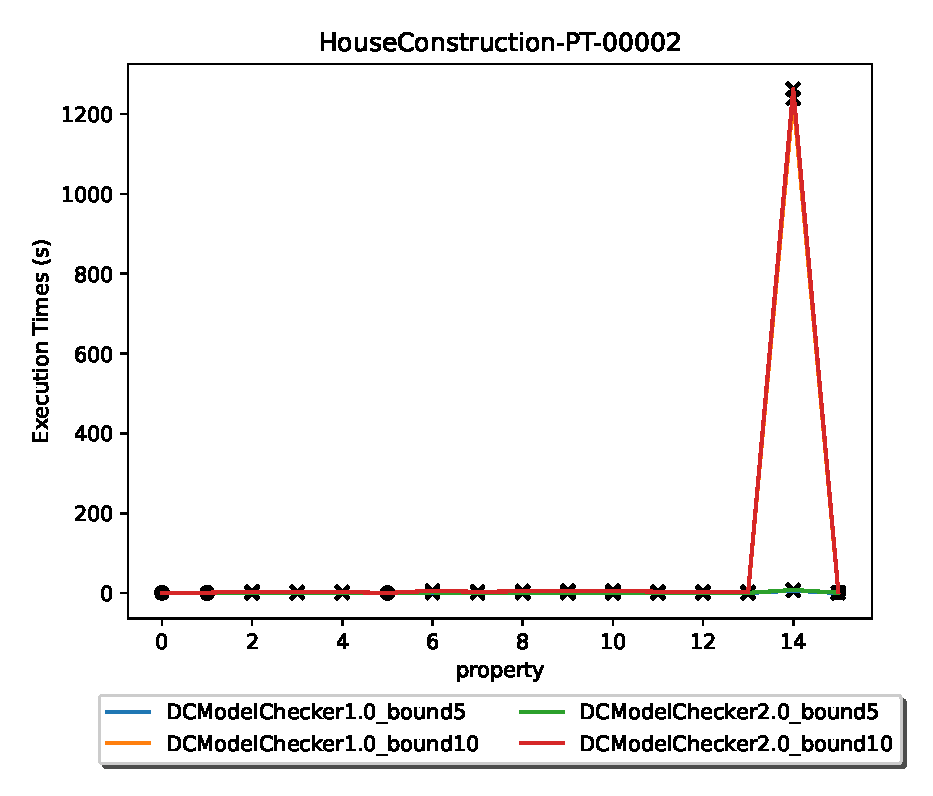
\includegraphics[width=.5\linewidth]{figures/FCPlots/HouseConstruction-PT-00002_FCPlot.eps} &
    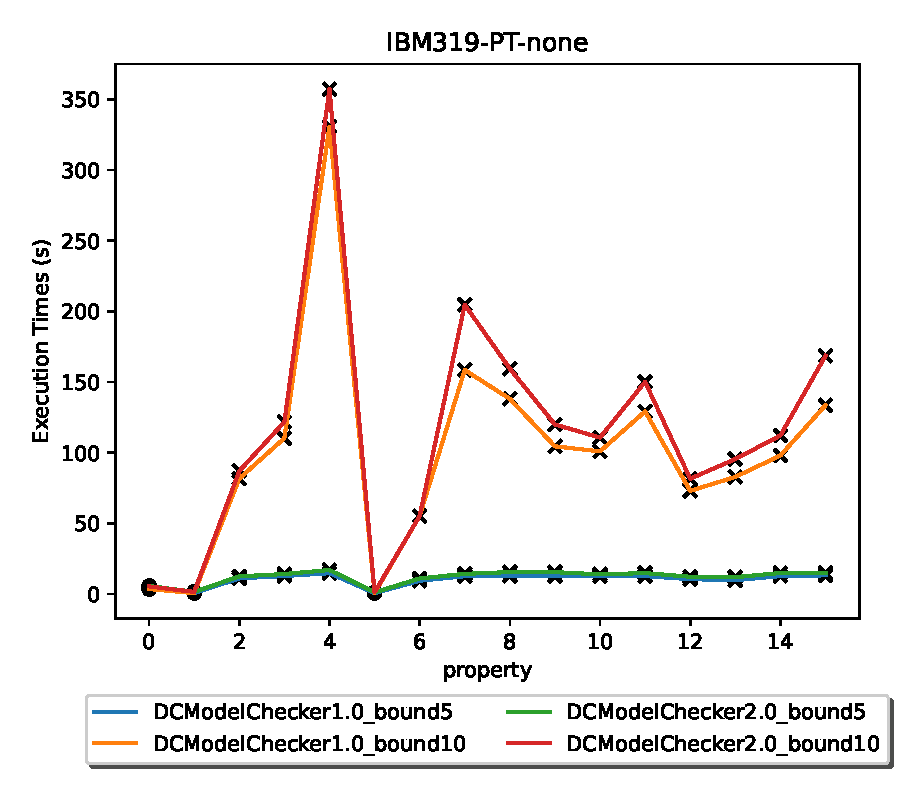
\includegraphics[width=.5\linewidth]{figures/FCPlots/IBM319-PT-none_FCPlot.eps}  \\
   %\includegraphics[width=.5\linewidth]{figures/FCPlots/HypercubeGrid-PT-C3K4P4B12_FCPlot.eps}\\
 \end{tabular}    
  %row
  %\begin{tabular}{cc}
  % \includegraphics[width=.5\linewidth]{figures/FCPlots/HypertorusGrid-PT-d2k1p8b00_FCPlot.eps} &
  %  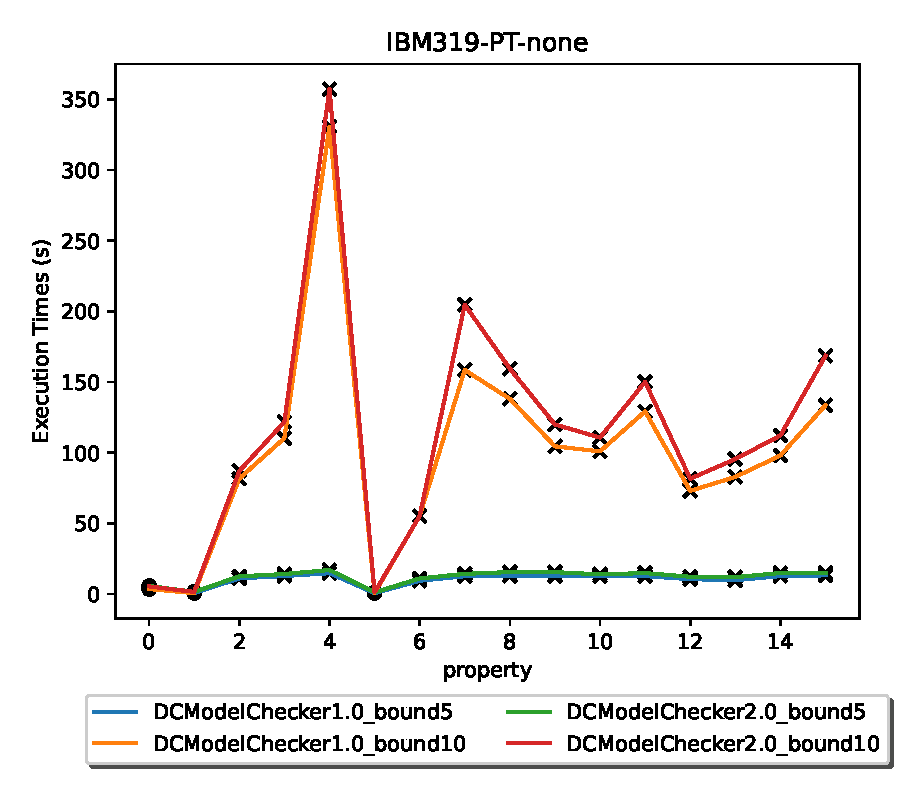
\includegraphics[width=.5\linewidth]{figures/FCPlots/IBM319-PT-none_FCPlot.eps}  \\
 %\end{tabular}    
\end{table}

\begin{table}[]
 %Row5
 \begin{tabular}{cc}
  \includegraphics[width=.5\linewidth]{figures/FCPlots/IBM703-PT-none_FCPlot.eps}&
   \includegraphics[width=.5\linewidth]{figures/FCPlots/IBM5964-PT-none_FCPlot.eps} \\
\end{tabular}    
   %
   \begin{tabular}{cc}
    \includegraphics[width=.5\linewidth]{figures/FCPlots/IOTPpurchase-PT-C01M01P01D01_FCPlot.eps}  &
    \includegraphics[width=.5\linewidth]{figures/FCPlots/Kanban-PT-00005_FCPlot.eps}\\
\end{tabular}    
\end{table}


\begin{table}[]
\begin{tabular}{cc}
   \includegraphics[width=.5\linewidth]{figures/FCPlots/MAPK-PT-00008_FCPlot.eps} &
    \includegraphics[width=.5\linewidth]{figures/FCPlots/PaceMaker-PT-none_FCPlot.eps}  \\
 \end{tabular}    


 %Row7
 \begin{tabular}{cc}
  \includegraphics[width=.5\linewidth]{figures/FCPlots/SimpleLoadBal-PT-02_FCPlot.eps}&
  \includegraphics[width=.5\linewidth]{figures/FCPlots/TCPcondis-PT-05_FCPlot.eps}  \\
\end{tabular}    
\begin{tabular}{cc}
\includegraphics[width=.5\linewidth]{figures/FCPlots/TriangularGrid-PT-1200_FCPlot.eps}&
  \includegraphics[width=.5\linewidth]{figures/FCPlots/CircularTrains-PT-012_FCPlot.eps}\\

\end{tabular}
\end{table}

\newpage
\subsection{Experiment 3: Verification of Unbounded Petri nets}\label{exp:upn}
To quote Amat et al, ``It is difficult to find benchmarks for unbounded Petri nets''~\cite{AmatDH22}. The strength of DCModelChecker 2.0 lies in verifying unbounded Petri nets. Since, MCC benchmarks are bounded~\cite{AmatDH22}, we make use of the unbounded Petri nets given by~\cite{NAmatGH} and verify LTLFireability properties in comparison with DCModelChecker 1.0~\cite{Zen2DBMC}, ITS-Tools~\cite{ITSMCC}. The results of these experiments are in Table~\ref{table:unboundedpn}, and~\cite{Zen2DBMC}. Each property that was verified is false. In each case it was observed that DCModelChecker 2.0 and DCModelChecker 1.0 returned that the property is false and additionally gave a counterexample trace, whereas ITS-Tools and Tapaal~\cite{DavidJJJMS12} returned that the property is false. Here, we compared our tools against both ITS-Tools and Tapaal, since Tapaal is faster than ITS-Tools and we give a comparative perspective of our tool's performance. In Section~\ref{exp:upn}, we verified LTLFireability properties of unbounded Petri nets which were all found to be false (while specifying the bound as $5$).
The properties are described in Table~\ref{table:upnprop}. The detailed output is available in the artifact~\cite{Zen2DBMC}.

\begin{table}[ht]
    \centering
    \resizebox{0.7\columnwidth}{!}{

        \begin{tabular}{|c|c|c|c|c|}
            \hline
            \multirow{2}{*}{Model} & \multicolumn{4}{c|}{Execution Times(ms)}                                                   \\
            \cline{2-5}
                                   & DCModelChecker 1.0   (bound =5)                    & DCModelChecker 2.0 (bound =5) & ITS-Tools & Tapaal         \\
            \hline
            Parity                 & \textbf{0.010}                           & 0.40               & 0.933     & 0.02           \\
            \hline
            PGCD                   & \textbf{0.019}                           & 0.98               & 1.487     & 0.07           \\
            \hline
            Process                & 0.033                                    & 0.85               & 1.201     & \textbf{1e-05} \\
            \hline
            CryptoMiner            & 0.036                                    & 0.64               & 0.957     & \textbf{7e-06} \\
            \hline
            Murphy                 & 0.031                                    & 0.83               & 1.161     & \textbf{8e-06} \\
            \hline
        \end{tabular}
    }
    \caption{Results of Experiment 3}
    \label{table:unboundedpn}

\end{table}

\begin{table}
    \centering

    \begin{tabular}{|l|l|}
        \hline
        \textbf{Model} & \textbf{Property}                 \\
        \hline
        Parity         & $\neg(t_0 U t_1)$                 \\
        \hline
        PGCD           & $\neg GF(t_0 U t_1)$              \\
        \hline
        Process        & $\neg F(t_0 U t_1)$               \\
        \hline
        CryptoMiner    & $\neg F(\text{OB } U \text{ GH})$ \\
        \hline
        Murphy         & $\neg F(t_1 U t_4)$               \\
        \hline
    \end{tabular}
    \caption{Experiment 3: List of properties verified on unbounded nets}
    \label{table:upnprop}

\end{table}
\subsection{Experiment 4: Verification of invariants for unbounded client-server systems using DCModelChecker 2.0}\label{exp:aps}

We have additionally verified client-server properties specified in the {\LC} language on our synthetic benchmark APS, against {\LC} specifications. These cannot be verified using DCModelChecker 1.0~\cite{Zen2DBMC}. The specifications are available in our artifact~\cite{Zen2DBMCv2}. Our experiments demonstrate that DCModelChecker 2.0 has an advantage over DCModelChecker 1.0 in being able to additionally verify invariants. And it can be added to the arsenal of BMC tools for Petri nets.
%In Section~\ref{sec:rel} we discuss the contributions of other tools that verify the properties of Petri nets.

\subsection{Related Petri net verification tools}
There are several tools such as KREACH~\cite{DixonL20}, Petrinizer~\cite{EsparzaLMMN14}, QCOVER~\cite{BlondinFHH16}, ICOVER~\cite{GeffroyLS18} verifying specific classes of properties like reachability and coverability of Petri nets. Recently, in~\cite{AmatBD21,AmatDH22} the generalized reachability of Petri net is encoded into a BMC problem and solved using SMT solvers. However, BMC for unbounded Petri nets with true concurrency and LTL properties while leveraging the power of SMT Solvers remained unexplored until now. DCModelChecker bridges this gap.


The MCC has attracted many tools for formal verification of concurrent systems that use a portfolio approach. In particular, we looked at ITS-Tools~\cite{ITSMCC} which implements structural reduction techniques~\cite{Mieg20} and uses a layer of SMT when solving LTL. Moreover, it does not perform BMC. While ITS-Tools is much faster on bounded nets (MCC benchmarks) it gives only binary answers (sat or unsat). From our experiments, on a subset of unbounded nets, while Tapaal is faster, it also gives binary answers. On the contrary, our tool preserves the original Petri net structure and additionally gives a counterexample trace which is useful in bug finding in systems.

\subsubsection*{Conclusion}\label{ssec:conclltltool}
In this chapter, we discussed the first of its kind verification tool for checking properties of unbounded client server systems using $2D$-BMC.

In Experiment 1 (Sec.~\ref{exp:compits}) where we compute the tool confidence as well as verify LTLFireability properties, we compare against only ITS-Tools since (at the time of experimentation) ITS-Tools was the MCC winner in the LTL Fireability category. Since the purpose of this experiment was to evaluate the tool confidence, it would not make any difference to compare against more than one tool, apart from the winning tool. In Experiment 3 (Sec.~\ref{exp:upn}) where we verify unbounded Petri nets which is not a category in the contest, we compared our tools against both ITS-Tools and Tapaal, since Tapaal is faster than ITS-Tools and we give a comparative perspective of our tool's performance.

We would like to have an optimal encoding of the PN with true concurrent semantics, such that we can better understand the advantage of true concurrent semantics. This will be done as part of future work.

Next, we shall look at an extension of the Petri net, called $\nu$-net and a different and richer logic, a variant of First Order logic, to express a different set of specifications of unbounded client server systems in the upcoming chapter.